\section{Actor Model} 

In previous work~\cite{gledhill2013modelinguas}, we represented each {\em actor}, human or autonomous component, of the WiSAR search team as a Mealy state machines as has been done in other models~\cite{bolton2013litreview}. This work uses Moore machines where output is determined only by present state.

\begin{comment}
\begin{figure}[h]
\center
\setlength{\abovecaptionskip}{1mm}
\setlength{\belowcaptionskip}{1mm}
\setlength{\textfloatsep}{1mm}
\setlength{\floatsep}{1mm}
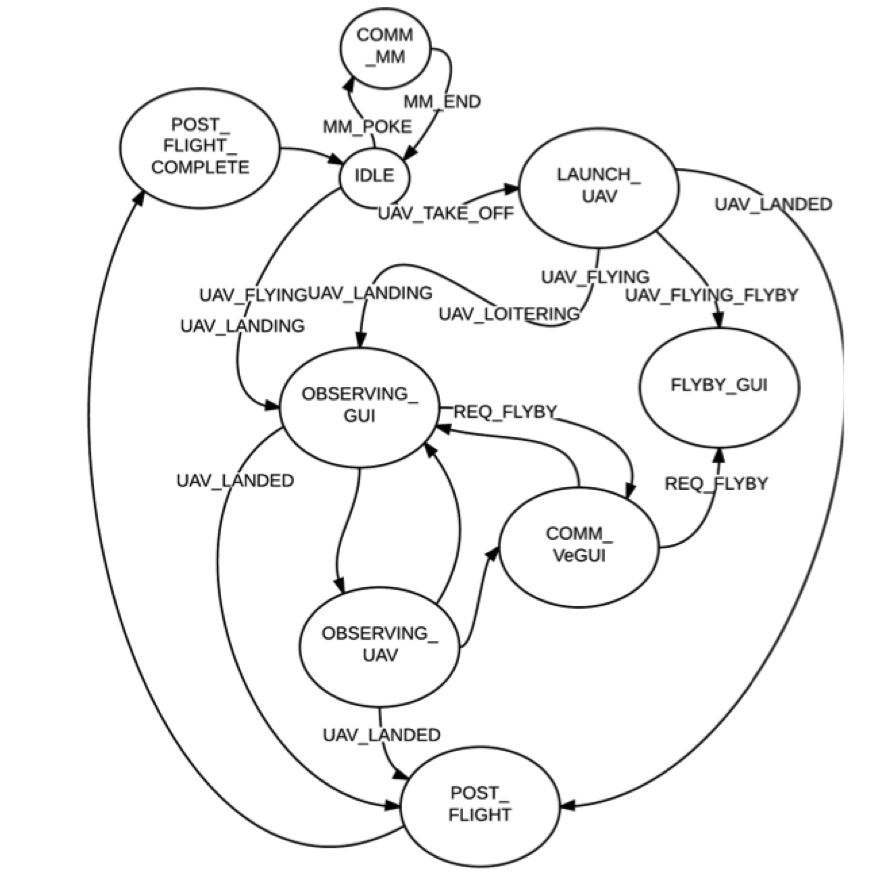
\includegraphics[height=2.4in]{DiRG.png}
\caption{Example actor model from prior work.}
\label{fig:dirg}
\end{figure}
\end{comment}

Actors represent the human decision-makers and autonomous elements of the WiSAR team.  An actor is composed of a set of states $S$, an initial state $s_0$, a set of inputs from the environment $\Sigma_{\rm env}$, a set of inputs from other actors on the team $\Sigma_{\rm team}$, a set of outputs $\Lambda_{\rm out}$, a simple form of memory $\Omega_{\rm men}$, and a transition function that determines the next state from the inputs and memory $\delta$. Formally, we denote an actor as:
\begin{equation}
 	Actor = (S, s_0, \Sigma_{\rm env}, \Sigma_{\rm team}, \Lambda_{\rm out}, \Omega_{\rm mem},\delta)
 \label{eq:actor}
 \end{equation}

 An actor's output has two components: signals to other actors on a team and a {\em duration} parameter that represents the time required for the actor to complete its transition to the next state.  Thus, $\Lambda_{\rm out}=\Sigma_{\rm team} \times \mathbb{N}^+$.
Relative task difficulty is expressed by the duration of the transition.
%The duration represents the relative difficulty of the task(s) associated with the transition.
We justify this by assuming that all tasks are performed at a constant rate, thus more difficult tasks take longer.
 A transition is a relation on the cross product of inputs with outputs where the brackets separate inputs from outputs.
\begin{equation}
 \delta:[S\times\Sigma_{\rm env}\times\Sigma_{\rm team}\times\Omega_{\rm mem}] \times [S\times \Sigma_{\rm team} \times \Omega_{\rm mem}], 
\end{equation} 
 
Given an actor's current state, set of input signals, and memory, it is possible for multiple transitions to be possible.  This occurs because we assume that multiple environment signals or inter-actor signals may be occurring at the same time, which are all perceived by the actor since we assume perception is a parallel operation.  Thus, it is useful to explicitly note the number of transitions that are possible from a given state.   A transition is considered {\em enabled} when all of its input
requirements are met and {\em disabled} otherwise. 

When an actor is in a given state, it is useful to explicitly denote the set of enabled and disabled transitions.  This information enables an estimate of algorithmic workload, where we assume that algorithmic workload is a function of the number of choices available to the actor.  Thus, we allow the current state to give a workload signal
\begin{equation}
	s_0^{\rm work\  sig} = (T_{enabled}, T_{disabled}) : T_{enabled} \cap T_{disabled} = \emptyset
 \label{eq:state}
\end{equation}

Internal variables within an actor are comprised of facts stored by an actor and used in decision making.
%Internal facts stored by an actor and used in decision making take the form of internal variables within an actor.
A good example of this can be seen in the mission manager actor of our simulation. As the search begins, the mission manager receives a number of data items from the parent search, e.g. search area and target description. These items of information need to be communicated separately to different actors, so they must be stored internally in the mean time. 
